% !TEX root = ../main.tex
\section{针对非抢占式排队系统的静态调度模型}
	\subsection{模型的假设与标记}
		\subsubsection{假设}
			\begin{enumerate}
				\item\label{抢占}RGV确定一次作业指令后中途不能放弃。例如选择RGV移动,CNC就绪三格距离后,RGV移动,CNC就绪过程中即使接收到临近CNC需求指令,也不能选择停下;一旦开始RGV上下料,CNC上下料或清理,直到结束才可以进行其它操作;
				\item\label{静态调度}RGV在完成一项作业任务后,立即判别执行下一个作业指令。此时,如果没有接到其他的作业指令,则RGV就在原地等待直到下一个作业指令;
				\item\label{机器周期1}假设RGV上下料,CNC上下料为一次完整的动作。例如在初始时,CNC为空闲状态,也需执行完整的RGV上下料,CNC上下料动作,但不会输出熟料,也无需RGV清洗,CNC加工;
				\item\label{机器周期2}考虑到信号接发时间的短暂性,因此忽略信号发送、接收时间;
				\item\label{机器周期3}考虑到传送带独立运动的可能性,假设传送带始终保证等待上料的CNC正前方有生料,供RGV上料工作;
			\end{enumerate}
		\subsubsection{标记}
			\begin{table}[htbp]
				\centering
				\caption{标记:针对非抢占式排队系统的静态调度模型}
				\label{标记:针对非抢占式排队系统的静态调度模型}
				\begin{longtabu}to\linewidth{@{}X[c]|X[l]@{}}
					\toprule
					变量&定义\\\midrule
					\(T_\mathrm{RGV}\)&RGV机器周期\\
					\(T_\mathrm{ready}\)&RGV等待时间\\
					\(T_\mathrm{move}\)&RGV移动时间\\
					\(T_\mathrm{update}\)&RGV\&CNC上下料时间\\
					\(T_\mathrm{clean}\)&RGV清洗时间\\
					\(T_\mathrm{CNC}\)&CNC机器周期\\
					\(T_\mathrm{wait}\)&CNC等待时间\\
					\(T_\mathrm{machine}\)&CNC加工时间\\
					\(t_\mathrm{max}\)&作业时间\\
					\(t\)&当前时间\\\bottomrule
				\end{longtabu}
			\end{table}
	\subsection{模型的建立与求解}
		\subsubsection{建立}
			\begin{figure}[htbp]
				\centering
				\caption{排队系统分类}
				\label{排队系统分类}
				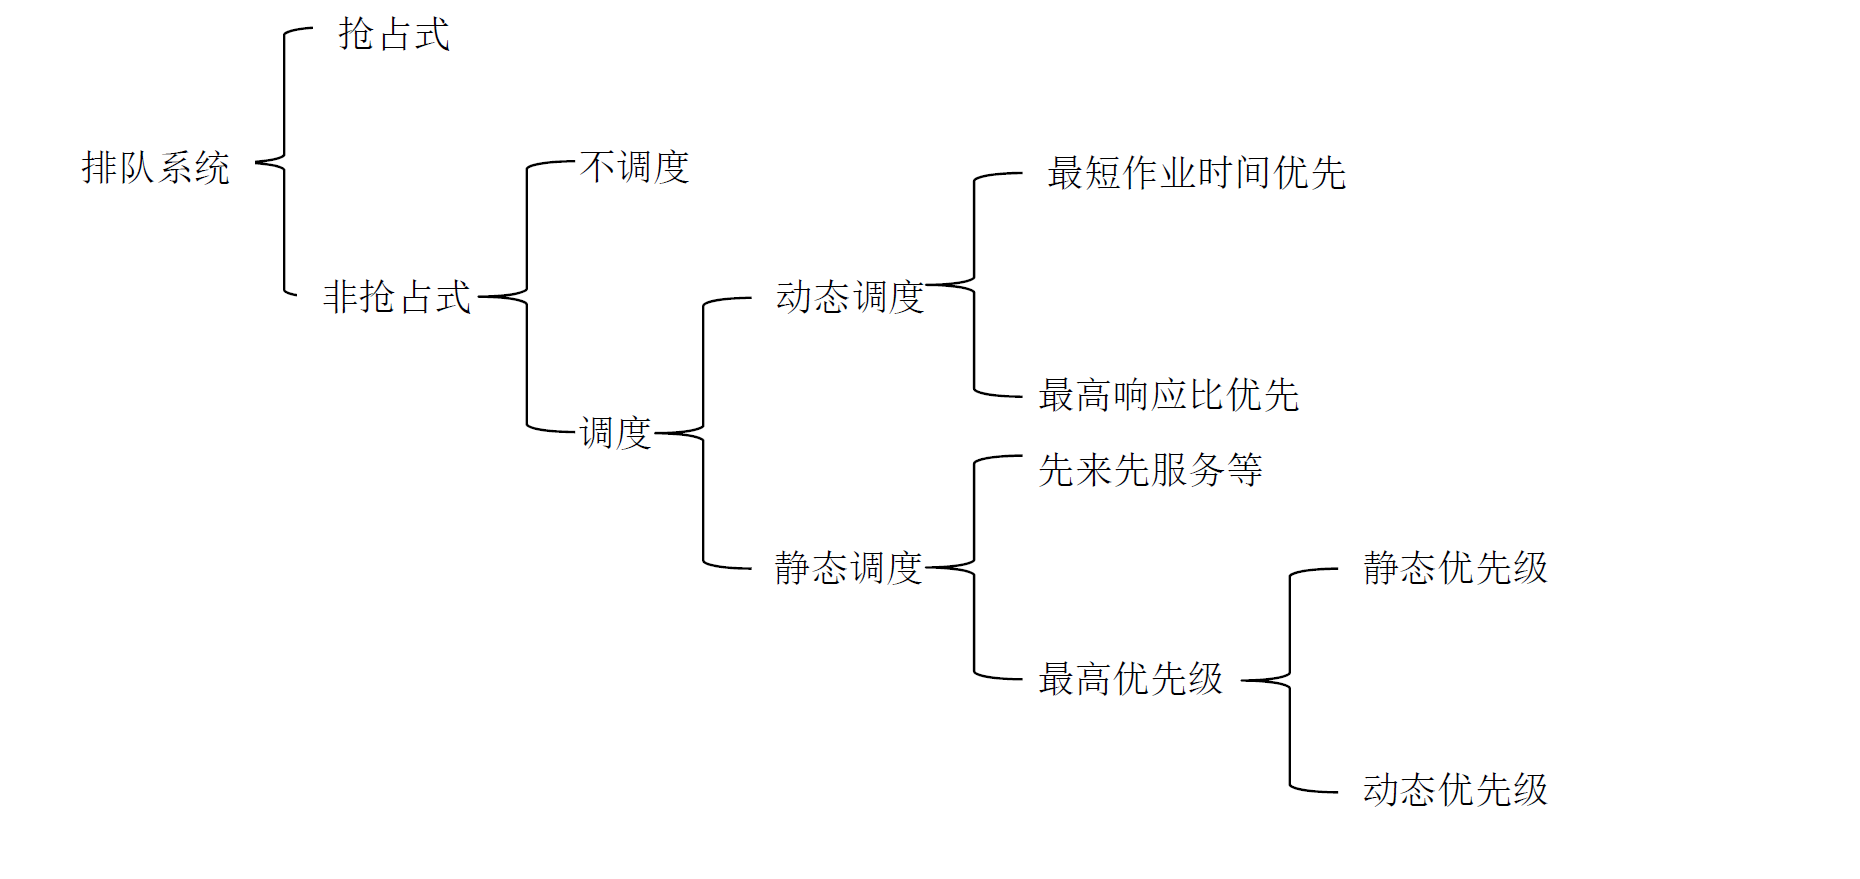
\includegraphics[width=10cm]{graph/classify.png}
			\end{figure}
			如图\ref{排队系统分类},排队系统根据服务是否可被暂停分为抢占式排队系统和非抢占式排队系统。根据假设\ref{抢占},该系统不允许抢占。
			\par\indent 针对非抢占式排队系统,通常会通过任务调度来提高服务效率。调度分为静态调度与动态调度。区别在于动态调度中RGV能预测每个CNC的加工完成时间从而预先进行移动或其他操作。根据假设\ref{静态调度},该系统只允许使用静态调度算法进行优化。
			\par\indent 针对本题,我们先求出局部最优解,将其作为初始解,再利用启发式算法进行全局寻优。全局寻优收敛解作为局部最优解的更替与检验,即若其解质量更高,则替代初始解,否则检验了局部最优解的合理性\cite{李睿智-400}。
			\par\indent 针对局部最优解的确定,常见排队模型包括电梯、磁盘寻道、操作系统等,对应的静态调度算法分别为先来先服务算法(FCFS)、最短寻道优先算法(SSF)、电梯扫描算法(Scan)和循环电梯扫描算法(CScan)。
			\par\indent 针对全局最优解的求取,启发式算法包括模拟退火算法、遗传算法、蚁群算法等。
			\begin{description}
				\item[遗传算法]能够进行并行搜索,搜索广度和随机性强,但易过早收敛于局部最优解;
				\item[蚁群算法]采用正反馈机制利于逼近全局最优解,但多样性的随机搜索导致了运算量过大;
				\item[模拟退火算法]\cite{钟志峰张田田-398}采用全局概率性搜索,具有良好的全局寻优性能、避免落入局部最优解,且鲁棒性强、简单易行。
			\end{description}
			\par\indent 因此我们最终选用模拟退火算法进行全局优化。
			\begin{figure}[htbp]
				\centering
				\begin{minipage}[htbp]{6cm}
					\centering
					\caption{先来先服务算法}
					\label{先来先服务算法}
					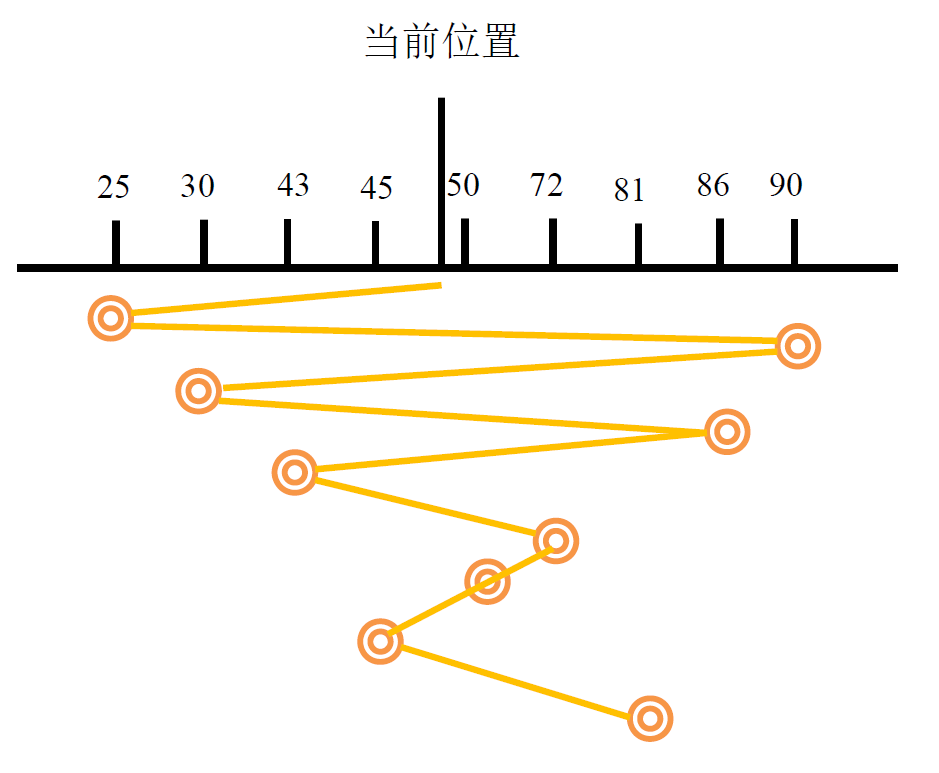
\includegraphics[width=6cm]{graph/FCFS.png}
				\end{minipage}
				\begin{minipage}[htbp]{6cm}
					\centering
					\caption{ 最短路径优先算法}
					\label{ 最短路径优先算法}
					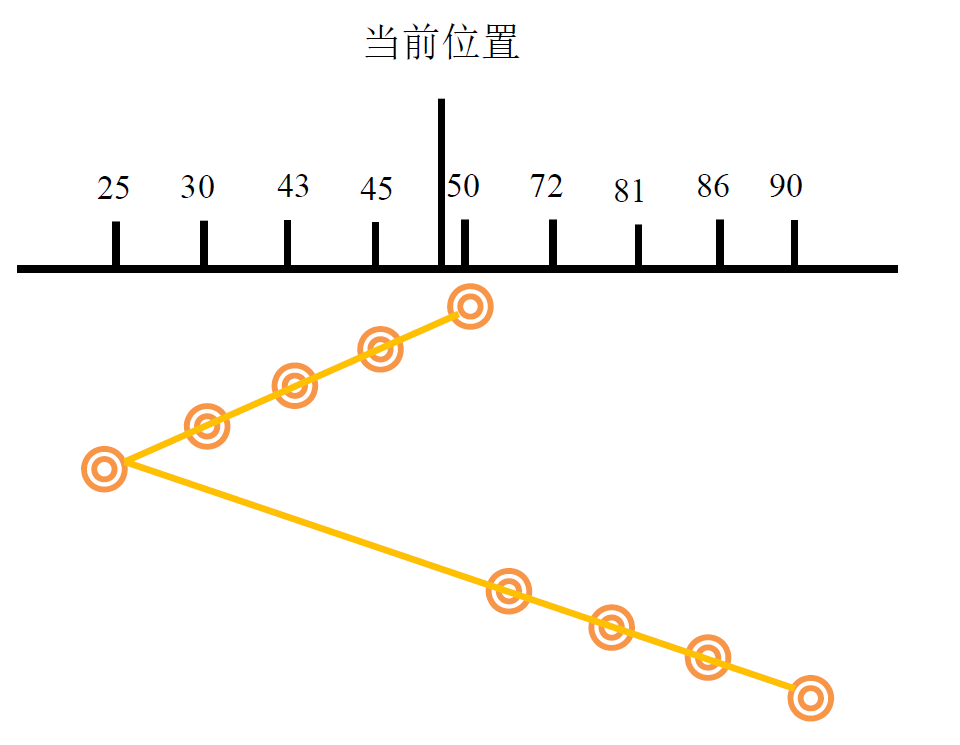
\includegraphics[width=6cm]{graph/SSF.png}
				\end{minipage}
			\end{figure}
			\begin{figure}[htbp]
				\centering
				\begin{minipage}[htbp]{6cm}
					\centering
					\caption{电梯扫描算法}
					\label{电梯扫描算法}
					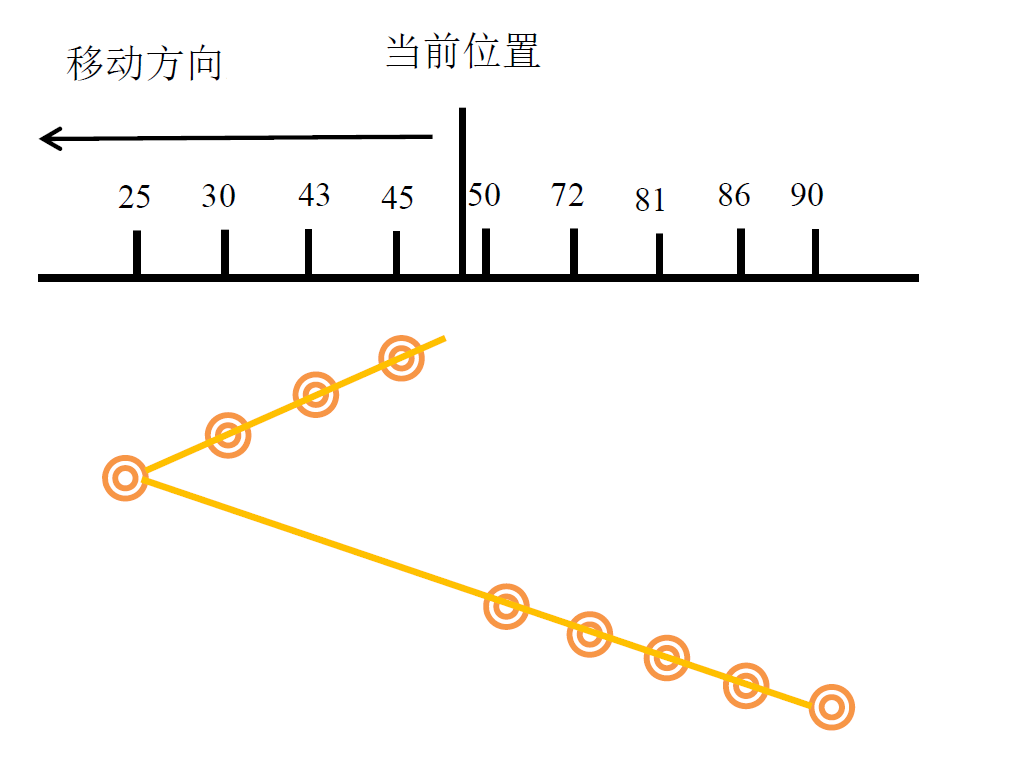
\includegraphics[width=6cm]{graph/Scan.png}
				\end{minipage}
				\begin{minipage}[htbp]{6cm}
					\centering
					\caption{循环电梯扫描算法}
					\label{循环电梯扫描算法}
					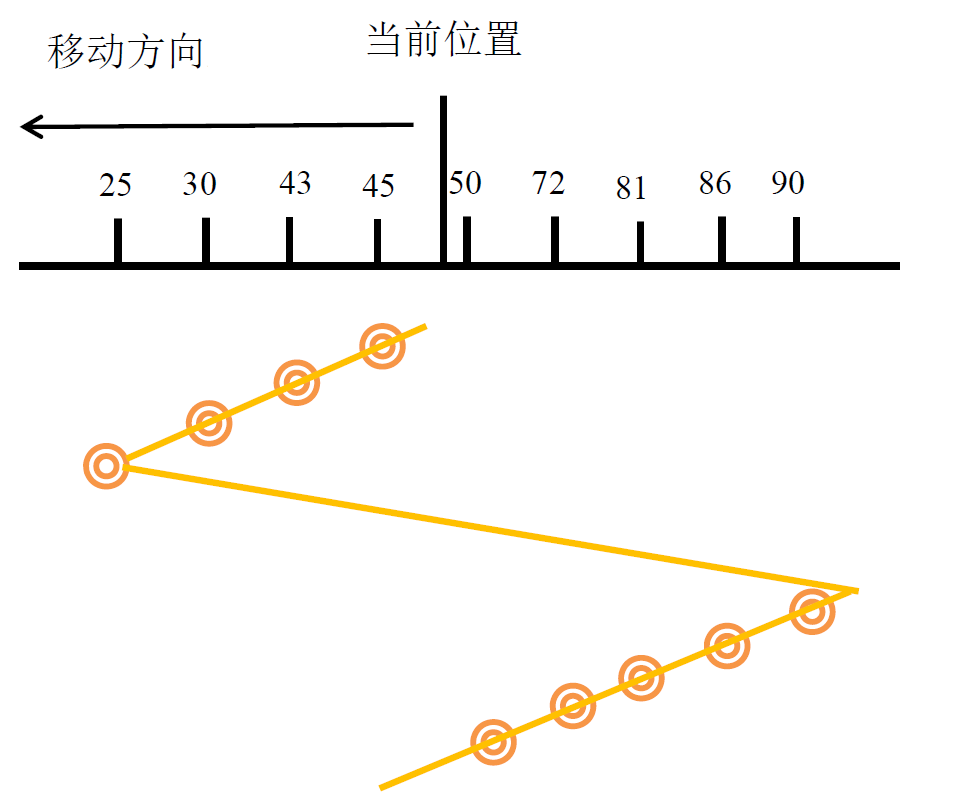
\includegraphics[width=6cm]{graph/CScan.png}
				\end{minipage}
			\end{figure}
			\paragraph{先来先服务算法}如图\ref{先来先服务算法},按请求的先后顺序,判断服务的先后顺序。平均RGV移动,CNC就绪距离大,用处比较少的一种算法。
			\paragraph{ 最短路径优先算法}如图\ref{ 最短路径优先算法},每次先满足和当前距离最近的请求,但无法保证平均寻道距离最短。
			\paragraph{电梯扫描算法}如图\ref{电梯扫描算法},可以防止“饥饿”\footnote{一个可运行的进程尽管能继续执行,但被调度器无限期地忽视,而不能被调度执行的情况。},减少平均等待时间,对所有CNC而言是一种比较公平的算法。
			\paragraph{循环电梯扫描算法}如图\ref{循环电梯扫描算法},扫描算法的变形,但RGV移动方向不会变化。当RGV移动到最外道时,立即返回服务最里面的CNC。
				\par\indent 将本系统类比计算机的批量处理操作系统\cite{石栋文瑾-399},定义类比概念。轨道式自动引导车RGV相当于中央处理器CPU,而数控机床CNC相当于等待CPU处理的进程。为了使操作系统的吞吐量尽可能的大,操作系统要考虑一定的进程调度策略。当多个进程同时请求CPU处理时,会根据特定的算法计算服务的顺序,即等待队列、依次进行服务。
				\begin{figure}[htbp]
					\centering
					\caption{机器周期}
					\label{机器周期}
					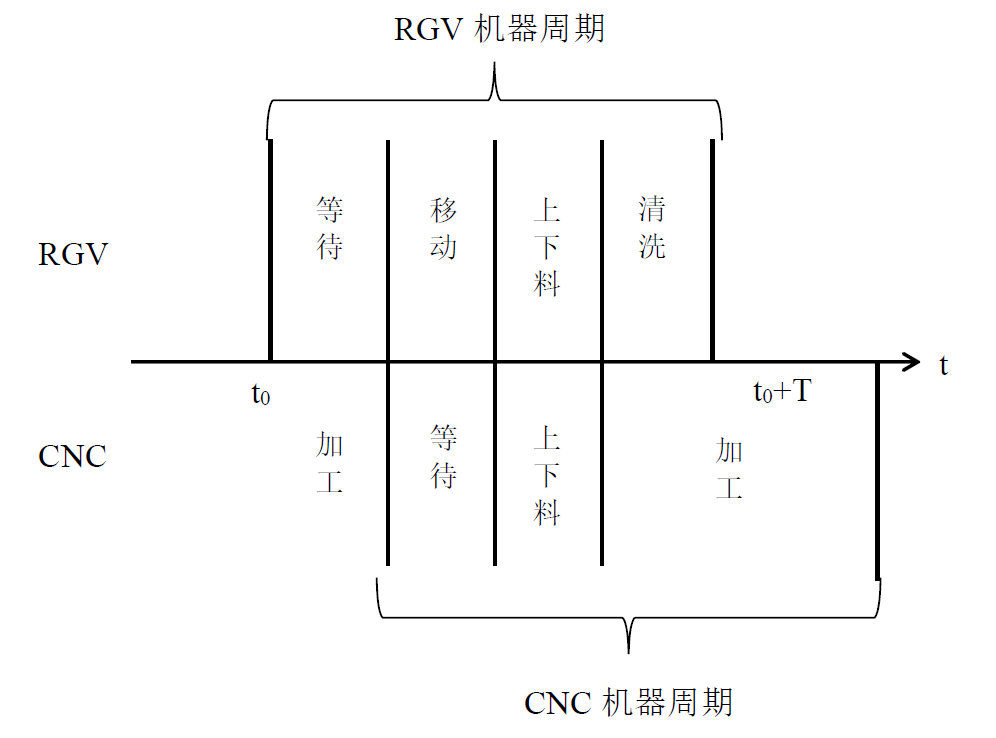
\includegraphics[width=10cm]{graph/periodStatic.png}
				\end{figure}
				\begin{align}
					\label{机器周期公式}
					T_\mathrm{RGV} & =T_\mathrm{ready}+T_\mathrm{move}+T_\mathrm{update}+T_\mathrm{clean} \\
					T_\mathrm{CNC} & =T_\mathrm{wait}+T_\mathrm{update}+T_\mathrm{machine}
				\end{align}
				\par\indent 如图\ref{机器周期},CPU执行时间以机器周期为单位。如图\ref{机器周期}。根据假设\ref{机器周期1}、\ref{机器周期2}和\ref{机器周期3},针对本题,如公式\ref{机器周期公式},RGV机器周期只包括等待、移动、上下料和清洗时间。清洗结束,成料总数加1。为方便计算成料总数,以清洗结束作为RGV机器周期的分界。
				\par\indent 相应的,CNC机器周期包括就绪、RGV上下料,CNC上下料和加工的时间。以CNC加工完成发出信号为CNC机器周期的分界。
				\par\indent 特别地,对于第一次加工的CNC,在上下料的时候不会有熟料输出,所以应在程序中设置一个标志位,记录每个CNC是否可输出熟料。初始时所有CNC标志位都为0。如果某一轮循环时该CNC不可输出熟料,则该轮RGV清理时间清0,标志位置1,熟料总数不变。否则按正常周期计算。
				\begin{figure}[htbp]
					\centering
					\caption{程序流程图:针对非抢占式排队系统的静态调度模型}
					\label{程序流程图:针对非抢占式排队系统的静态调度模型}
					\begin{tikzpicture}[align = center, node distance = 1.5cm]
						\node(开始)[startstop]{开始};
						\node(循环开始)
						[	process,
							below of = 开始
						]{循环开始};
						\node(是否有CNC发出信号?)
						[	decision,
							below of = 循环开始,
							yshift = -.5cm
						]{是否\\有CNC发出\\信号?};
						\node(等待)
						[	process,
							right of = 是否有CNC发出信号?,
							xshift = 3cm,
							yshift = 2cm
						]{等待};
						\node(有多个CNC发出信号;调用调度算法计算将被服务的CNC)
						[	io,
							below of = 是否有CNC发出信号?,
							yshift = -.5cm
						]{有多个CNC发出信号;\\调用调度算法计算将被服务的CNC};
						\node(RGV移动,CNC就绪)
						[	process,
							below of = 有多个CNC发出信号;调用调度算法计算将被服务的CNC
						]{RGV移动,CNC就绪};
						\node(RGV上下料,CNC上下料)
						[	process,
							below of = RGV移动,CNC就绪
						]{RGV上下料,CNC上下料};
						\node(RGV清洗,CNC加工)
						[	process,
							below of = RGV上下料,CNC上下料
						]{RGV清洗,CNC加工};
						\node(成品数加1,CNC增加1个机器周期)
						[	io,
							below of = RGV清洗,CNC加工
						]{成品数加1,\\CNC增加1个机器周期};
						\node(是否超时?)
						[	decision,
							below of = 成品数加1,CNC增加1个机器周期
						]{是否超时?};
						\node(时间增加1个RGV机器周期,刷新CNC冷却时间)
						[	process,
							left of = 循环开始,
							xshift = -3cm
						]{时间增加1个RGV机器周期,\\刷新CNC冷却时间};
						\node(结束)
						[	startstop,
							below of = 是否超时?
						]{结束};
						\draw[arrow](开始)--(循环开始);
						\draw[arrow](循环开始)--(是否有CNC发出信号?);
						\draw[arrow](是否有CNC发出信号?)-|node[right]{否}(等待);
						\draw[arrow](等待)--(循环开始);
						\draw[arrow](是否有CNC发出信号?)--node[right]{是}(有多个CNC发出信号;调用调度算法计算将被服务的CNC);
						\draw[arrow](有多个CNC发出信号;调用调度算法计算将被服务的CNC)--(RGV移动,CNC就绪);
						\draw[arrow](RGV移动,CNC就绪)--(RGV上下料,CNC上下料);
						\draw[arrow](RGV上下料,CNC上下料)--(RGV清洗,CNC加工);
						\draw[arrow](RGV清洗,CNC加工)--(成品数加1,CNC增加1个机器周期);
						\draw[arrow](成品数加1,CNC增加1个机器周期)--(是否超时?);
						\draw[arrow](是否超时?)-|node[left]{否}(时间增加1个RGV机器周期,刷新CNC冷却时间);
						\draw[arrow](时间增加1个RGV机器周期,刷新CNC冷却时间)--(循环开始);
						\draw[arrow](是否超时?)--node[right]{是}(结束);
					\end{tikzpicture}
				\end{figure}
				\par\indent 程序流程如图\ref{程序流程图:针对非抢占式排队系统的静态调度模型}。终止循环的条件是超时,如公式\ref{超时},当前时间再加一个RGV机器周期大于作业时间。
				\begin{align}
					\label{超时}
					t\leqslant t_\mathrm{max}\leqslant t+T_\mathrm{RGV}
				\end{align}
		\subsubsection{求解}
			代码见程序清单\ref{主程序}。该程序一共有6个参数可以输入,其中静态调度算法可以选择以下算法:
			\begin{enumerate}
				\item 先来先服务+最短路径优先\footnote{在程序开始运行时所有CNC被视为同时到达,所以有必要再加上别的算法计算优先次序。};
				\item 最短路径优先;
				\item 电梯扫描;
				\item 循环电梯扫描;
				\item 先来先服务+静态优先级;
				\item 静态优先级。
			\end{enumerate}
			\par\indent 除此之外可以选择动态调度的最短作业时间优先和不调度。并可以指定静态优先级。除此之外对于接下来的2道工序的情况和有概率发生故障的情况提供了可输入的相应参数。运行结果的一个示例见运行结果\ref{主程序结果}。
			\par\indent 程序清单\ref{穷举搜索最优静态优先级排序}给出了静态优先级算法的最优解。但计算时间较长,且结果略次于电梯扫描算法,并不适用。求解结果见运行结果\ref{穷举搜索最优静态优先级排序结果}。
			\par\indent 程序清单\ref{模拟退火搜索最优静态调度和最优CNC工序分配分布的主程序}和\ref{模拟退火搜索最优静态调度和最优CNC工序分配分布}给出了一个求解最优静态调度的启发式算法。
			\par\indent 程序的具体说明看注释及断言\footnote{判断并提示程序输入是否合法的语句。}。
	\subsection{模型的检验与分析}
		\subsubsection{分析}
			对于排队系统,除了静态调度外还有动态调度和不调度的随机输入。动态调度由于能预先根据进程的完成时间进行调度,往往能取得比静态调度更好的结果。通常这是静态调度所能达到的上界。
			\begin{figure}[htbp]
				\centering
				\caption{动态调度的机器周期}
				\label{动态调度的机器周期}
				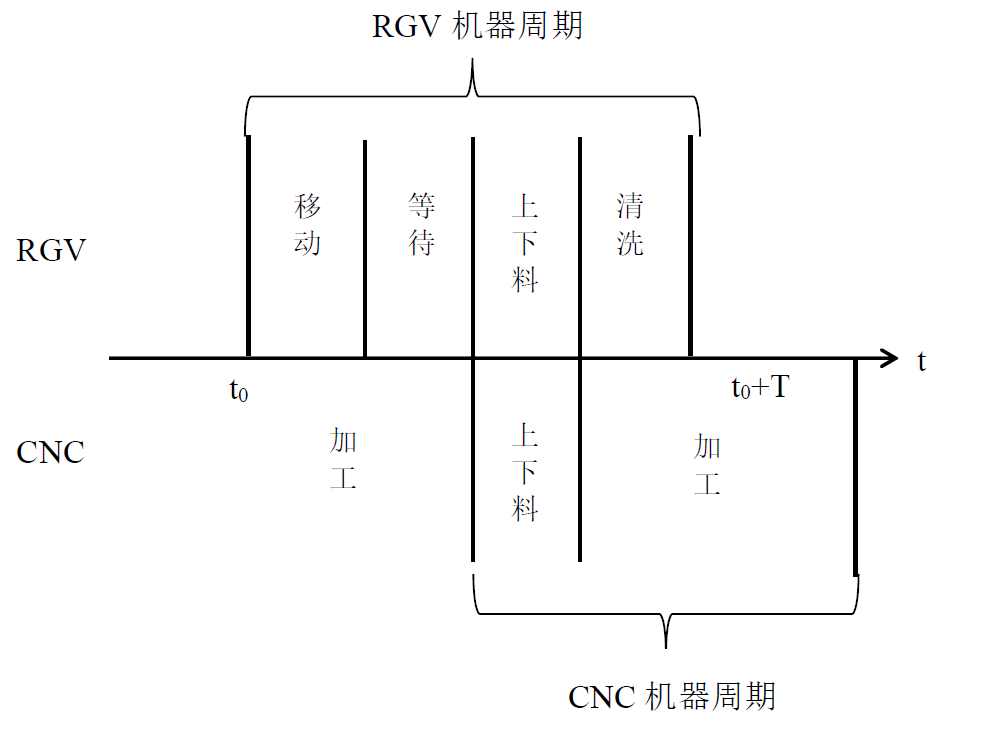
\includegraphics[width=8cm]{graph/periodDynamic.png}
			\end{figure}
			\par\indent 例如最短作业时间优先算法(SJF),如图\ref{动态调度的机器周期}和公式\ref{动态调度的机器周期公式},RGV计算出接下来一个CNC最先加工完成,从而在该CNC加工完成之前先移动该CNC所在位置等待。从而该CNC无需等待RGV移动过来。节省了CNC的等待时间。
			\begin{align}
				\label{动态调度的机器周期公式}
				T_\mathrm{RGV} & =T_\mathrm{move}+T_\mathrm{ready}+T_\mathrm{update}+T_\mathrm{clean} \\
				T_\mathrm{CNC} & =T_\mathrm{update}+T_\mathrm{machine}
			\end{align}
			\par\indent 以第1组数据为例。可见最优的静态调度算法和最短作业时间优先算法已经相差不多。
			\begin{table}[htbp]
				\centering
				\caption{3种调度情况的比较}
				\label{3种调度情况的比较}
				\begin{longtabu}to\linewidth{@{}X[c]|*3{X[c]}@{}}
					\toprule
					\diagbox{指标}{结果}{情况}&不调度(随机服务)&静态调度(最优)&动态调度(SJF)\\\midrule
					熟料总数&163	&369	&376	\\\bottomrule
				\end{longtabu}
			\end{table}
